\section{Case Study: Key-Value Store}
\label{sec:kvs}
In this section, we present two variants of a key-value store (KVS) implemented
using Bloom. We begin with an abstract protocol that any key-value store will
satisfy, and then provide both single-node and replicated implementations of
this protocol. We then introduce a graphical visualization of the dataflow in a
Bloom program, and use this visualization to reason about the \emph{points of
  order} in our programs: places in the program where additional coordination
may be required to guarantee consistent results (Section~\ref{sec:calm}).

\subsection{Abstract Key-Value Store Protocol}

\begin{figure}[t]
\begin{scriptsize}
\begin{lstlisting}
module KVSProtocol
  def state
    interface input, :kvput, 
      ['client', 'key', 'reqid'], ['value']
    interface input, :kvget, ['reqid'], ['key']
    interface output, :kvget_response, 
      ['reqid'], ['key', 'value']
  end
end
\end{lstlisting}
\centering
\vspace{-10pt}
\caption{Abstract key-value store protocol.}
\label{fig:kvs-proto}
\end{scriptsize}
\vspace{-2pt}
\end{figure}

Figure~\ref{fig:kvs-proto} specifies a protocol for interacting with an abstract
key-value store. The protocol comprises two input interfaces (representing
attempts to insert and fetch items from the store) and a single output interface
(which represents the outcome of a fetch operation). To use an implementation of
this protocol, a Bloom program can store key-value pairs by inserting facts into
\texttt{kvput}. To retrieve the value associated with a key, the client program
inserts a fact into \texttt{kvget} and then looks for the corresponding response
tuple in \texttt{kvget\_response}. In both cases, the client program must supply
a unique request identifier (\texttt{reqid}) to differentiate tuples in the
event of multiple concurrent requests.

A module which uses a key-value store but is indifferent to the specifics of the
implementation may simply mix in this protocol specification and postpone
committing to a particular implementation until runtime. As we will see shortly,
an implementation of the KVSProtocol is a collection of Bud rules that read
tuples from the protocol's input interfaces and send results to the output
interface.

\subsection{Single-Node Key-Value Store}
\label{sec:simple-kvs}
\begin{figure}[t]
\begin{scriptsize}
\begin{lstlisting}
module BasicKVS
  include KVSProtocol

  def state
    table :kvstate, ['key'], ['value'] (*\label{line:kvs-state}*)
  end

  declare
  def do_put
    kvstate <+ kvput.map{|p| [p.key, p.value]} (*\label{line:kvs-put}*)
    prev = join [kvstate, kvput], [kvstate.key, kvput.key] (*\label{line:kvs-join}*)
    kvstate <- prev.map{|b, p| b} (*\label{line:kvs-clean}*)
  end

  declare
  def do_get
    getj = join [kvget, kvstate], [kvget.key, kvstate.key] (*\label{line:kvs-getjoin}*)
    kvget_response <= getj.map do |g, t|
      [g.reqid, t.key, t.value]
    end
  end
end
\end{lstlisting}
\centering
%%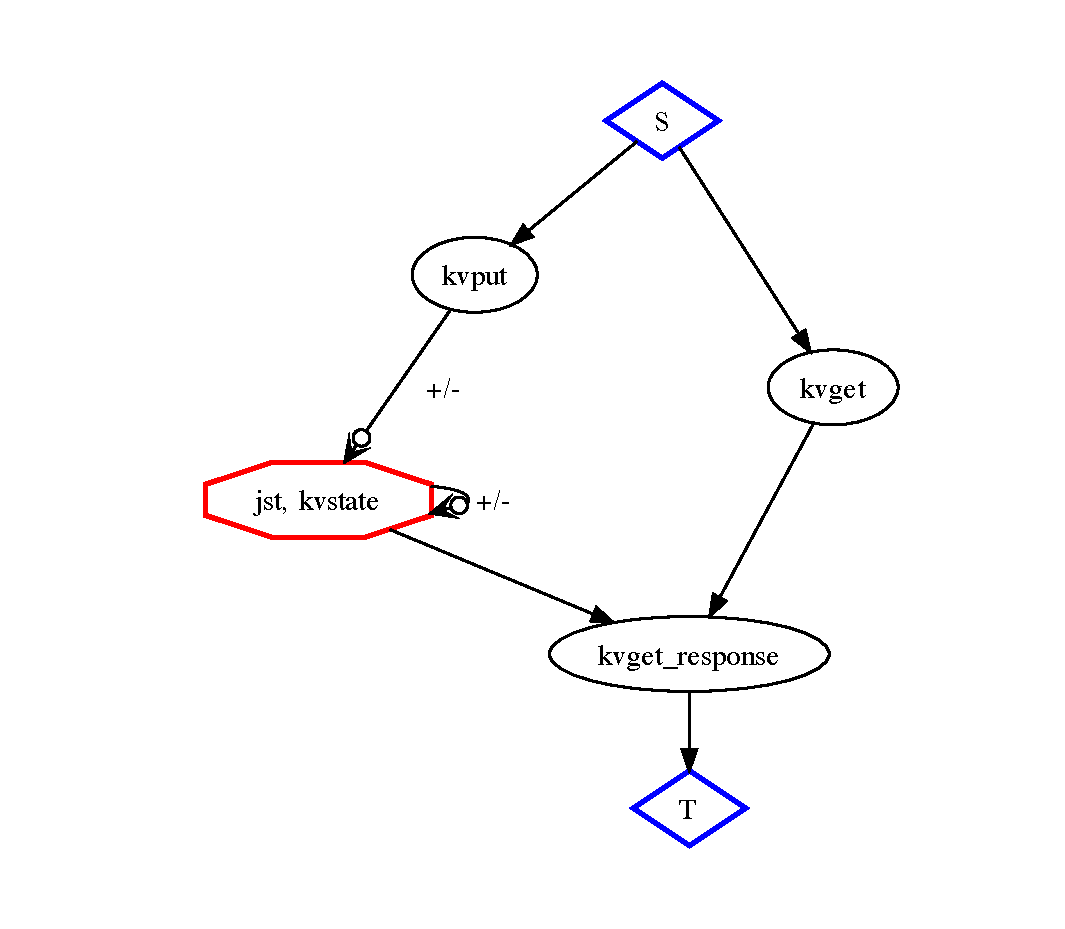
\includegraphics[width=0.55\linewidth]{fig/basickvs.pdf}
\vspace{-10pt}
\caption{Single-node key-value store implementation.}
\label{fig:kvs-impl}
\end{scriptsize}
\vspace{-2pt}
\end{figure}

Figure~\ref{fig:kvs-impl} contains a simple single-node implementation of the
abstract key-value store protocol. Key-value pairs are stored in a persistent
table called \texttt{kvstate} (line~\ref{line:kvs-state}). When a \texttt{kvput}
tuple appears, its key-value pair is stored in \texttt{kvstate} at the immediately
following timestep (line~\ref{line:kvs-put}).  If the given key already exists in
\texttt{kvstate}, we want to replace the key's old value. This is done by
joining \texttt{kvput} against the current version of \texttt{kvstate}
(line~\ref{line:kvs-join}). If a matching tuple is found, the old key-value pair
is removed from \texttt{kvstate} at the beginning of the next timestep
(line~\ref{line:kvs-clean}). Note that we also insert the new key-value pair
into \texttt{kvstate} in the next timestep (line~\ref{line:kvs-put});
hence, we implement an overwriting update as an atomic deletion and insertion.

\subsection{Replicated Key-Value Store}
\label{sec:rep-kvs}

\begin{figure}[t]
\begin{scriptsize}
\begin{lstlisting}
module ReplicatedKVS
  include BasicKVS
  include MulticastProtocol

  def state
    interface input, :kvput, (*\label{line:rep-put-beg}*)
      ['client', 'key', 'reqid'], ['value']  (*\label{line:rep-put-end}*)
  end

  declare
  def replicate
    send_mcast <= kvput.map do |k| (*\label{line:send-mcast-beg}*)
      unless members.include? [k.client]  (*\label{line:not-rep}*)
        [k.reqid, [@addy, k.key, k.reqid, k.value]]   (*\label{line:marshall}*)            
      end
    end (*\label{line:send-mcast-end}*)
  end

  declare
  def apply_put
    kvput <= mcast_done.map{|m| m.payload}  (*\label{line:mcast-done}*)

    kvput <= pipe_chan.map do |d| (*\label{line:mcast-peer-beg}*)
      if d.payload.fetch(1) != @addy
        d.payload
      end
    end (*\label{line:mcast-peer-end}*)
  end
end
\end{lstlisting}
\vspace{-10pt}
\caption{Replicated key-value store implementation.}
\label{fig:kvs-repl}
\end{scriptsize}
\vspace{-2pt}
\end{figure}

Next, we extend the basic key-value store implementation to support replication
(Figure~\ref{fig:kvs-repl}). To communicate between replicas, we use a simple
multicast library implemented in Bloom; the complete source code for this
library can be found in Appendix~\ref{app:network-code}. To send a multicast, a
program inserts a fact into \texttt{send\_mcast}; a corresponding fact appears
in \texttt{mcast\_done} when the multicast is complete.\footnote{XXX: error
  handling.} The multicast library also exports the membership of the multicast
group in a table called \texttt{members}.

Our replicated key-value store is implemented on top of the single-node
key-value store described in the previous section. When a new key is inserted by
a client, we multicast the insertion to the other replicas
(lines~\ref{line:send-mcast-beg}--\ref{line:send-mcast-end}). To avoid repeated
multicasts of the same inserted key, we avoid multicasting updates we receive
from another replica (line~\ref{line:not-rep}). We apply an update to our local
\texttt{kvstate} table in two cases: (1) if a multicast succeeds at the node
that originated it (line~\ref{line:mcast-done}) (2) whenever a multicast is
received by a peer replica
(lines~\ref{line:mcast-peer-beg}--\ref{line:mcast-peer-end}).

Note that the implementation of ReplicatedKVS wants to ``intercept''
\texttt{kvput} events from clients, and only apply them to the underlying
BasicKVS module when certain conditions are met. To achieve this, we
``override'' the declaration of the \texttt{kvput} input interface
(lines~\ref{line:rep-put-beg}--\ref{line:rep-put-end}). In ReplicatedKVS,
references to \texttt{kvput} appearing in the lhs of rules are resolved to the
\texttt{kvput} provided by BasicKVS, while references in the rhs of rules
resolve to the local \texttt{kvput}.  This is unambiguous, because a module
cannot insert into its own input or read from its own output
interfaces. Nevertheless, the current syntax for achieving this is somewhat
cryptic; it might be improved by the addition of a namespace-like concept.
\paa{we probably don't want to say this.  the idea of the above is that it
is ``sugar'' for implicit namespaces.  another option would be to make them
explicit.}

\subsection{Predicate Dependency Graphs}
\begin{figure}[t]
\centering
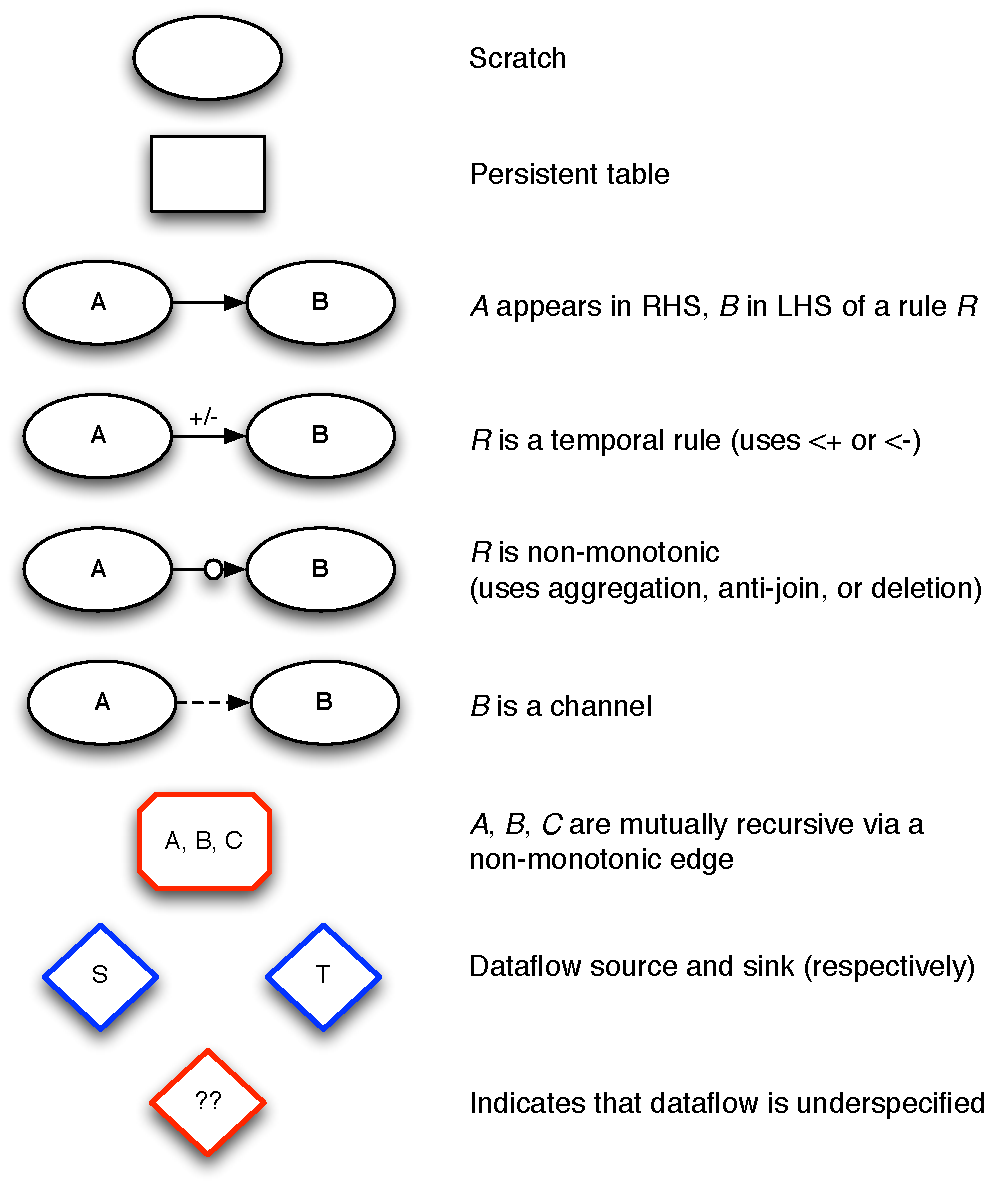
\includegraphics[width=0.9\linewidth]{fig/mittalk_legend.pdf}
\vspace{-10pt}
\caption{Visual analysis legend.}
\label{fig:analysis-legend}
\vspace{-2pt}
\end{figure}

Now that we have introduced two concrete implementations of the abstract
key-value store protocol, we turn to analyzing the properties of these
programs. We begin by describing the graphical dataflow representation used by
our analysis. In the next section, we discuss the dataflow graphs generated for
the two key-value store implementations.

A Bloom program may be viewed as a dataflow graph with external input interfaces
as sources, external output interfaces as sinks, collections as internal nodes,
and rules as edges. This graph represents the dependencies between the
collections in a program, and can be generated automatically by the Bud
interpreter. Figure~\ref{fig:analysis-legend} contains a list of the different
symbols and annotations in the graphical visualization; we provide a brief
summary below.

Each node in the graph is either a collection or a cluster of collections;
tables are shown as rectangles, ephemeral collections (scratch, periodic and
channel) are depicted as ovals, and clusters (described below) as octagons. A
directed edge from node $A$ to node $B$ indicates that $B$ appears in the lhs of
a Bloom rule that references $A$ in the rhs, either directly or through a join
expression. An edge is annotated based on the operator symbol in the rule. If
the rule uses the \texttt{$<$+} or \texttt{$<$-} operators, the edge is marked
with ``$+/-$''. This indicates that facts traversing the edge ``spend'' a
timestep to move from the rhs to the lhs. Similarly, if the rule uses the
\texttt{$<\sim$} operator, the edge is a dashed line---this indicates that facts
from the rhs appear at the lhs at a non-deterministic future time. If the rule
involves a non-monotonic operation (aggregation, anti-join, or the \texttt{$<$-}
operator), then the edge is marked with a white circle.  To make the
visualizations more readable, any strongly connected component marked with both
a circle and a $+/-$ edge is collapsed into an octagonal ``temporal cluster,''
which can be viewed abstractly as a single, non-monotonic node in the
dataflow. Any non-monotonic edge in the graph is a \emph{point of order}, as are
all edges incident to a temporal cluster, including any self-edges.

\subsection{Analysis}
Figure~\ref{fig:pdg-kvs-proto-analysis} presents a visual representation of the
abstract key-value store protocol. The diagram depicts the semantics implied by
the protocol's interfaces: data is inserted into the input interfaces
(\texttt{kvput} and \texttt{kvget}), and results eventually appear in the output
interface (\texttt{kvget\_response}). Naturally, the abstract protocol does not
specify a connection between the input and output events; this is indicated in
the diagram by the red diamond, which denotes an underspecified dataflow. A
concrete realization of the key-value store protocol must, at minimum, supply a
dataflow that connects an input interface to the output interface.

Figure~\ref{fig:pdg-kvs-analysis} shows the visual analysis of the single-node
KVS implementation, which supplies a concrete dataflow for the unspecified
component in the previous graph.  \texttt{kvstate} and \texttt{prev} are
collapsed into a red octagon because they are part of a strongly connected
component in the graph with both negative and temporal edges.  Any data flowing
from \texttt{kvput} to the sink must cross at least one non-monotonic point of
order (at ingress to the octagon) and possible an arbitrary number of them (via
the octagon's self-edge), and any path from \texttt{kvget} to the sink must join
state potentially affected by non-monotonicity (because \texttt{kvstate} is used
to derive \texttt{kvget\_response}).

Reviewing the code in Figure~\ref{fig:kvs-impl}, we see that this is
unavoidable.  The contents of \texttt{kvstate} at a given time are defined (in
part; line~\ref{line:kvs-clean}) in terms of its contents at the immediate
previous state and the current input.  Hence the state of \texttt{kvstate} at
any point in time may depend on the order of arrival of \texttt{kvput} tuples.
We challenge the reader to implement the KeyValueProto interface in a way that
has no such point of order.
\paa{I vote to keep the previous line, but am willing to be overridden.  
I am conjecturing that it isn't possible to implement a k/v store with the
desired replacing semantics without points of order (at least on kvget)}



\begin{figure}[t]
\centering
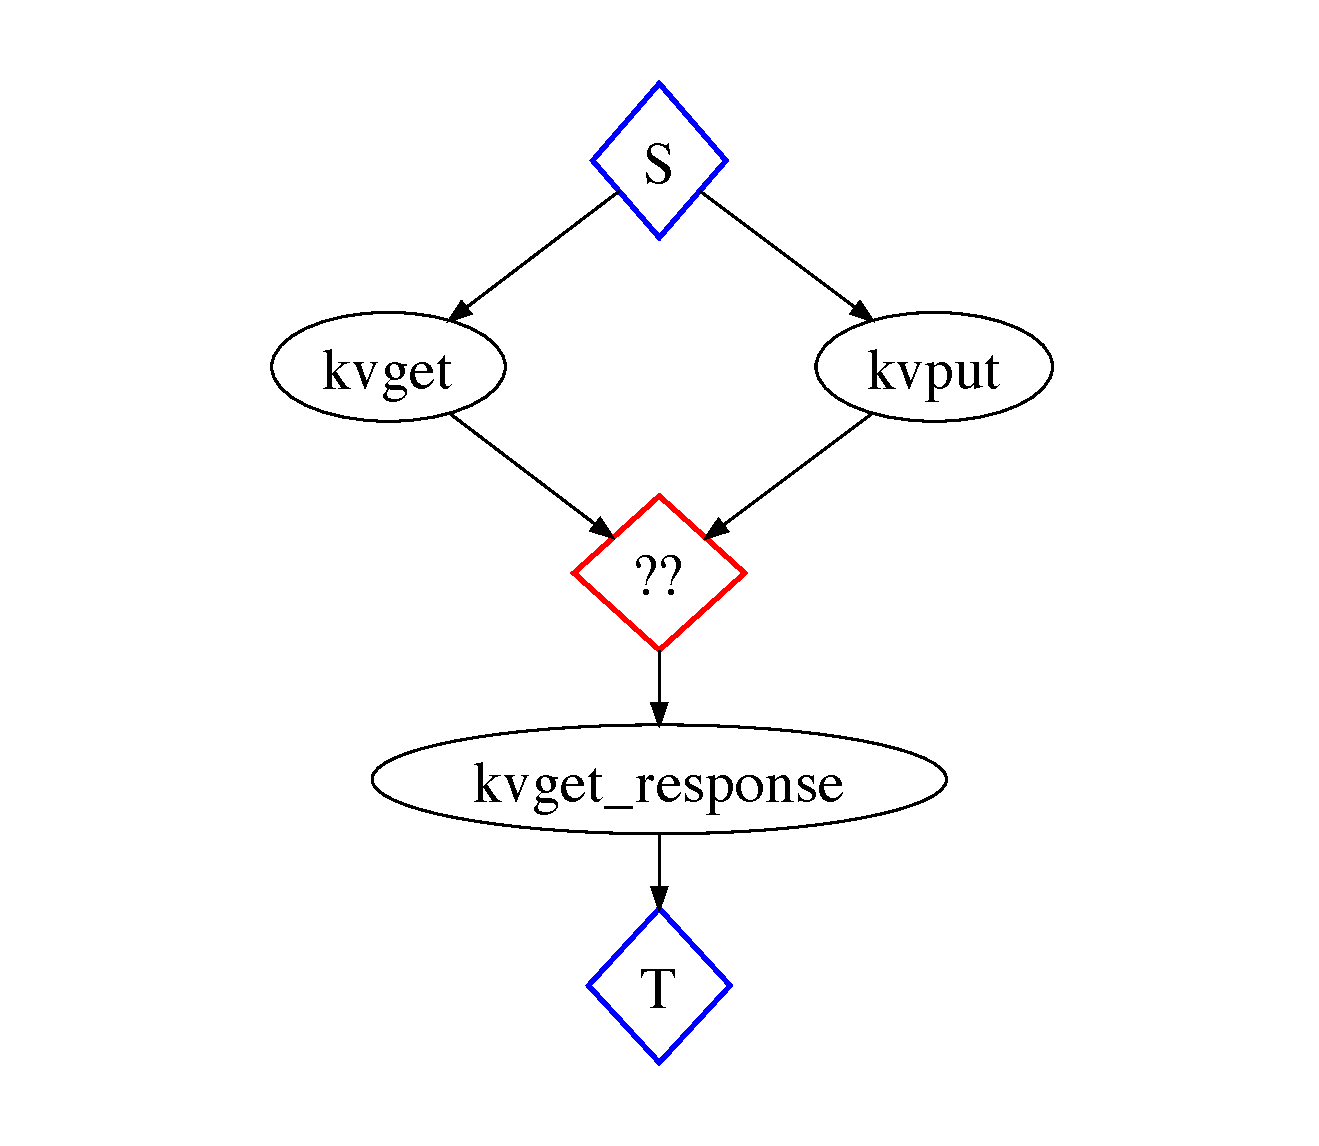
\includegraphics[width=0.8\linewidth]{fig/kvs_proto_pdg.pdf}
\vspace{-10pt}
\caption{Visualization of the abstract key-value store protocol.}
\label{fig:pdg-kvs-proto-analysis}
\vspace{-2pt}
\end{figure}

\begin{figure}[t]
\centering
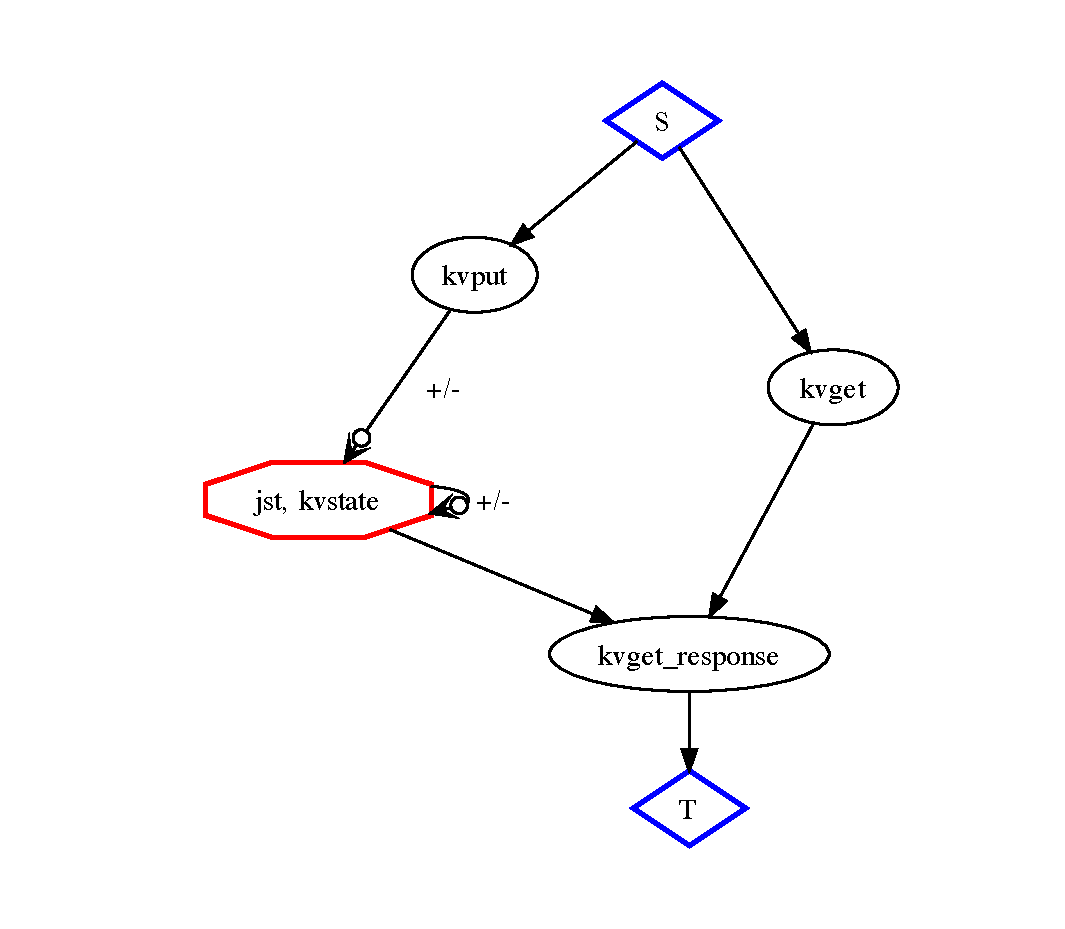
\includegraphics[width=0.9\linewidth]{fig/basickvs.pdf}
\vspace{-10pt}
\caption{Visualization of the single-node key-value store.}
\label{fig:pdg-kvs-analysis}
\vspace{-2pt}
\end{figure}
